\chapter{Regression Discontinuity Design}
\label{ch-reg-dis}

This chapter is based on
Ref.\cite{book-mixtape}.

This chapter assumes that the
reader has read Chapter \ref{ch-po}
on Potential Outcomes (PO).

In Regression Discontinuity Design (RDD),
one switches the treatment
dose $\rvd$ from 0 when $\rvx<\xi$ to 1 
where $\rvx>\xi$,  where  $\rvx$ is an
observed confounder (call
it the {\bf switch confounder})
and $\xi$ is a threshold value
for $\rvx$.
One measures the jump $\delta$
in the treatment outcome $\rvy$
as $\rvx$ passes through
$\rvx=\xi$.
Then one makes the
very reasonable assumption
that $\delta$ equals\footnote{
ATE, which stands for 
``average treatment effect",
is defined
in Chapter \ref{ch-po}.} 
 $\caly_{1|x=\xi}-
\caly_{0|x=\xi}=ATE_{|x=\xi}$
for an imaginary experiment in which
the confounder $\rvx$
acts as a normal confounder
that doesn't switch 
 the treatment dose $\rvd$.

For example,
$d^\s$
might be whether
an individual is admitted
to Harvard Univ., $y^\s$
might be how much
money
the individual earns for the first 20 years
after graduating from
Harvard, and $x^\s$
might be his SAT scores.
We assume Harvard only admits 
students with
an SAT score higher
than $\xi$.



\section{PO analysis}

\begin{figure}[h!]
$$
\begin{array}{ccc}
\xymatrix{
&\rvx^\s\ar[dr]\ar[dl]
\\
\rvd^\s\ar[rr]&&\rvy^\s
}
&&
\xymatrix{
&\rvx^\s=x\ar[dr]\ar[dl]
\\
\rvd^\s\ar[rr]&&\rvy^\s
}
\\
\\
G&&G_{disc}
\end{array}
$$
\caption{
2 bnets used in the
PO analysis of RDD. The 
TPMs for $G_{disc}$
are  defined in terms of the TPMs for
$G$. The TPM 
$P(d^\s|x^\s)$ 
for $G_{disc}$
is discontinuous in $x^\s$.}
\label{fig-reg-dis-bnets}
\end{figure}

The TPMs,
printed in blue,
for the 
bnet
$G_{disc}$
shown
in Fig.\ref{fig-reg-dis-bnets},
are as follows.
Note
that the
TPMs for the
bnet $G_{disc}$
are defined in 
terms
of the TPMs for the bnet $G$.



\beq \color{blue}
P(x^\s)=
\delta(x^\s, x)
\eeq

\beq \color{blue}
P(y^\s|d^\s, x^\s=x)=
P_{\rvy|\rvd, \rvx}(y^\s|d^\s, x)
\eeq

\beq \color{blue}
P(d^\s|x^\s=x)=
\left\{
\begin{array}{ll}
P_{\rvd|\rvx}(d^\s|x^\s=x)
& \text{ for } x>\xi
\\
\delta(d^\s, 0)
& \text{ for } x<\xi
\end{array}
\right.
\eeq

Define

\beq
E_{\s|x}[y^\s(\td)]=E_{y|x}[\rvy(\td)
]=\caly_{\td|x}
\eeq
and

\beq
\xi\pm = \xi \pm \eps
\eeq
for some infinitesimal $\eps>0$.

See Fig.\ref{fig-reg-dis}.
In RDD, we assume that
if we define the 
following
2 $\delta$'s, 
one for bnet
$G$ and the other
for bnet $G_{disc}$,
then the two $\delta$'s are 
equal,
and they equal
a conditional ATE.

\beq
\delta_{G_{disc}}=\caly_{1|x=\xi+} 
- \caly_{0|x=\xi-}
\eeq

\beq
\delta_{G}=\caly_{1|x=\xi} 
- \caly_{0|x=\xi}
\eeq

\beq
\delta_{G}=\delta_{G_{disc}}=\delta
\eeq


\beq
\delta= ATE_{|x=\xi}
\eeq


\begin{figure}[h!]
\centering
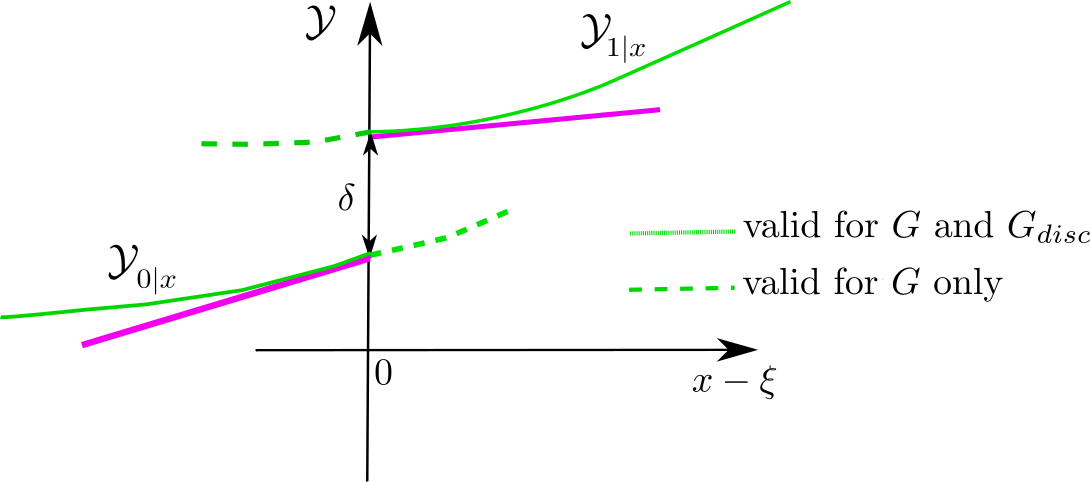
\includegraphics[width=4in]
{reg-dis/reg-dis.png}
\caption{
The jump $\delta$
between $\caly_{1|x}$
and $\caly_{0|x}$
is the same for $G$ and 
$G_{disc}$. 
} 
\label{fig-reg-dis}
\end{figure}



\section{Linear Regression}
In this
section,
we show how to apply
linear regression (LR)
to the PO analysis of RDD.


$y^\s$
can be fitted
as a function of $x\in \RR$,
for $\td^\s \in \bool$,
 as follows.
Here $\eps^\s$
is the residual
for individual $\s$
and $b_0, m_0, b_1, m_1\in \RR$
are the fit parameters.

\beq
y^\s = [b_0 + m_0(x-\xi)](1-\td^\s)
+  [b_1 + m_1(x-\xi)]\td^\s
+ \eps^\s
\;.
\label{eq-rdd-lr}
\eeq

Note that Eq.(\ref{eq-rdd-lr})
 yields a straight line
in the $y^\s-x$ plane
for $\td^\s=0$,
and another 
straight line for $\td^\s=1$.
These 2 lines are 
colored magenta in Fig.\ref{fig-reg-dis}.
We are
using the
standard symbols
$b$ to denote
the y-intercept, and $m$ 
to denote the slope
of a straight line.

Taking the expected value
of Eq.(\ref{eq-rdd-lr}), we get

\beq
\caly_{\td|x}=
[b_0 + m_0(x-\xi)](1-\td)
+  [b_1 + m_1(x-\xi)]\td
\;.
\eeq
Hence,

\beq
\caly_{1|x=\xi+}=b_1\;,\;\;
\caly_{0|x=\xi-}=b_0
\eeq

\beq
\delta= b_1-b_0
\eeq

